\documentclass[a4paper]{lipics-v2021}

\usepackage{amsmath,amssymb,amsfonts}
\usepackage{algorithmic}
\usepackage{graphicx}
\usepackage{textcomp}
\usepackage{xcolor}
\usepackage{tikz}
\usepackage{booktabs}
\usepackage{array}
\usetikzlibrary{arrows.meta,positioning,fit,backgrounds,shapes.geometric}

\setlength{\marginparwidth}{2cm}
\usepackage{todonotes}
\setlength{\emergencystretch}{3em}

\newcommand{\FIXME}[1]{{\color{blue} [TODO: #1]}}
\newcommand{\REF}[1]{{\color{red} [REF]}}
\newcommand{\TODO}[1]{{\color{blue} [@@ #1]}}
\newcommand{\todoS}[1]{\todo[author=Satish, inline,color=blue!25]{#1}}
\newcommand{\todoA}[1]{\todo[author=Alex, inline,color=red!15]{#1}}
\newcommand{\mypara}[1]{{\vspace{0.1mm}\noindent\textbf{#1}}}

\bibliographystyle{plainurl}

\title{Observability-Driven Intelligence for Anomaly Detection in
Cloud-Native Distributed Microservices}
\titlerunning{Observability-Driven AIOps for Cloud-Native Microservices}

\author{Ngoc Duc Anh Nguyen}
       {School of Built Environment, Engineering and Computing,
        Leeds Beckett University, Leeds, UK}
       {n.nguyen3896@leedsbeckett.ac.uk}
       {}{}

\author{Satish Kumar}
       {School of Built Environment, Engineering and Computing,
        Leeds Beckett University, Leeds, UK}
       {s.kumar@leedsbeckett.ac.uk}
       {}{}

\author{Nawar Jawad}
       {School of Built Environment, Engineering and Computing,
        Leeds Beckett University, Leeds, UK}
       {n.nawar@leedsbeckett.ac.uk}
       {}{}

\authorrunning{N.\,D.\,A. Nguyen, S. Kumar, and N. Jawad}

\Copyright{Ngoc Duc Anh Nguyen, Satish Kumar, and Nawar Jawad}

\ccsdesc[500]{Computer systems organization~Cloud computing}
\ccsdesc[300]{Computing methodologies~Anomaly detection}
\ccsdesc[300]{Information systems~Data management systems}

\keywords{anomaly detection, microservices, observability, machine learning,
Kubernetes, distributed tracing, root cause analysis, AIOps,
anti-money laundering}

\funding{This research is supported by Leeds Beckett University.}

\begin{document}

\maketitle
\begin{abstract}
Automated fault diagnosis in cloud-native microservice architectures remains an open
challenge: the three pillars of observability---metrics, logs, and distributed
traces---each capture a distinct failure dimension, yet most production AIOps
deployments exploit only one signal modality, leaving cross-modal causal chains
undetected until user-visible degradation occurs. We present an observability-driven
AIOps platform that closes this gap through continuous, fully offline multi-modal
intelligence, motivated by AML compliance environments where data residency
regulations categorically prohibit telemetry export to third-party infrastructure.
Eight Kubernetes-native AIOps services ingest a three-pillar telemetry pipeline
(Prometheus, Loki, Grafana Tempo) and apply a three-algorithm ML pipeline in
sequence: Isolation Forest anomaly scoring over 60-second stream-windowed feature
vectors, Pearson correlation root cause ranking over sliding observational windows,
and ordinary least-squares regression on p95 latency trends for predictive SLO breach
forecasting. Rather than delegating incident narration to a cloud-hosted model, the
platform synthesises MELT context through a locally deployed Qwen2.5-3B large
language model~\cite{qwen2024} served via Ollama~\cite{ollama2023} and
continuously fine-tuned with LoRA adapters~\cite{hu2022lora} on resolved incident
outcomes---producing structured, actionable JSON diagnostic reports with no external
API call leaving the cluster. The platform is evaluated through controlled Chaos Mesh~\cite{chaosmesh2020}
fault injection across four fault classes, addressing RQ1--RQ3. Results confirm
fault detection within two 60-second cycles, on-cluster LLM narration at 3--5
seconds per report, and zero telemetry egress over a 2-hour injection session---establishing the platform as both
a privacy-preserving operational tool and a reproducible experimental substrate for
quantitative AIOps evaluation.
\end{abstract}

% ── 1. INTRODUCTION ──────────────────────────────────────────────────────────
\section{Introduction}
\label{sec:introduction}

Distributed microservice architectures now coordinate hundreds of containerised
services across Kubernetes clusters, each emitting metrics, logs, and distributed
traces at sub-second resolution~\cite{burns2016borg}. Anomalies in such systems
manifest as subtle cross-service causal chains---a memory leak first inflects a
metric, propagates to trace latency shifts, and eventually cascades into error-log
floods---patterns invisible to any single-modal detector and intractable for human
operators at the telemetry volumes modern clusters produce.

In regulated domains such as anti-money laundering~(AML), this challenge is
compounded by data residency obligations. Financial regulations in most
jurisdictions explicitly prohibit exporting operational telemetry to third-party
cloud services~\cite{kosinska2023toward}, categorically excluding commercially
hosted AIOps platforms precisely in the environments where automated anomaly
detection is most consequential. AML workloads further exhibit architectural
heterogeneity---synchronous KYC REST~APIs, asynchronous Kafka event streams, and
stateful case-management workflows with legally mandated lifecycle invariants---that
generates telemetry across fundamentally different operational patterns
simultaneously.

Existing approaches are inadequate on two fronts. Rule-based monitors evaluate
individual metrics against static thresholds, generating excessive false-positive
alert volumes and failing on distributed cross-service anomalies~\cite{soldani2022anomaly}.
Supervised learning approaches require labelled training data unavailable for
novel failure modes. Commercial AIOps platforms---Dynatrace Davis~AI~\cite{dynatrace2023}
and Datadog Watchdog~\cite{datadog2023}---apply sophisticated correlation algorithms
but mandate continuous telemetry export to vendor-managed infrastructure. No existing
open-source platform unifies multi-modal anomaly detection, correlation-based RCA,
and predictive SLO forecasting as a privacy-preserving, fully offline
Kubernetes-native service.

We address this gap with two complementary design decisions: (i)~all intelligence
executes within the cluster---Isolation Forest~\cite{liu2012isolation} anomaly
scoring, Pearson correlation root cause ranking, OLS SLO breach prediction, and
Qwen2.5-3B~\cite{qwen2024} incident narration fine-tuned with
LoRA~\cite{hu2022lora} via Ollama~\cite{ollama2023}, with no external API access;
and (ii)~the AML testbed uses a transactional outbox pattern that dual-routes
domain events as both Kafka streams and OpenTelemetry span events carrying business
attributes, providing naturally labelled ground-truth anomaly signals without
secondary annotation.

The main contributions are: (i)~a production-grade, open-source eleven-service
Kubernetes platform for AML-domain observability with a fully offline intelligence
layer satisfying financial data residency requirements; (ii)~a domain event-based
instrumentation strategy deriving ground-truth anomaly labels from AML compliance
state transitions via OpenTelemetry span attributes; (iii)~a three-algorithm offline
ML pipeline (Isolation Forest, Pearson correlation RCA, OLS SLO prediction)
integrated with a locally fine-tuned Qwen2.5-3B served via Ollama; and (iv)~a
controlled Chaos Mesh fault injection evaluation protocol addressing signal
sufficiency~(RQ1), ML-driven RCA localisation~(RQ2), and distributed tracing
overhead on regulated workloads~(RQ3).

% ── 2. BACKGROUND ────────────────────────────────────────────────────────────
\section{Background and Related Works}
\label{sec:background}
\textit{\textcolor{blue}{We have space and please try to add max 25-30 references. It would be good to restore the old content sections.  }}
\subsection{Cloud-Native Observability}

Observability infers system state from telemetry and reconstructs failure
context~\cite{boten2022cloudnative}. Cloud-native applications emit three signal
classes: metrics (Prometheus~\cite{prometheus2015}), logs (Loki~\cite{loki2019}),
and distributed traces (Tempo~\cite{tempo2022}). Metrics capture resource and
latency trends, logs record events, and traces expose causal execution paths.

\begin{figure}[t]
\centering
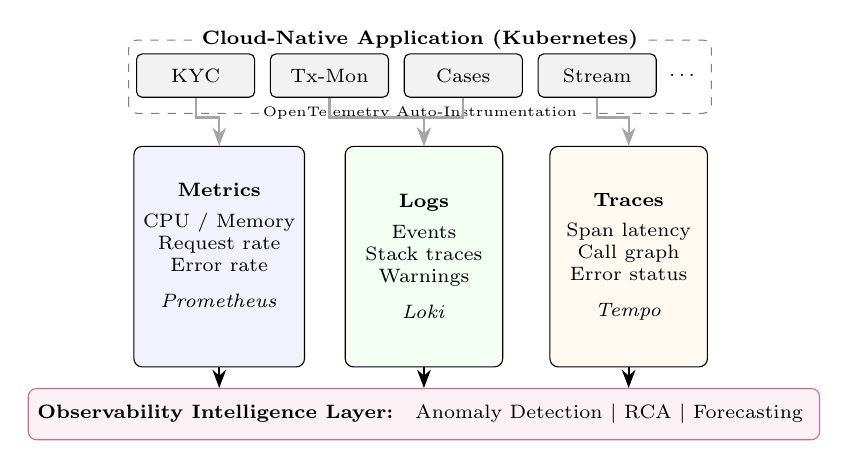
\begin{tikzpicture}[
  svc/.style={draw,rectangle,rounded corners=2pt,minimum height=0.55cm,
              minimum width=1.5cm,align=center,font=\scriptsize,fill=gray!10},
  pillar/.style={draw,rectangle,rounded corners=3pt,minimum height=2.8cm,
                 minimum width=2.0cm,align=center,font=\scriptsize},
  intel/.style={draw,rectangle,rounded corners=3pt,minimum height=0.65cm,
                align=center,font=\scriptsize},
  arr/.style={-Stealth,thick}
]
% Application layer
\node[svc] (s1) at (1.0,4.1) {KYC};
\node[svc] (s2) at (2.7,4.1) {Tx-Mon};
\node[svc] (s3) at (4.4,4.1) {Cases};
\node[svc] (s4) at (6.1,4.1) {Stream};
\node[font=\scriptsize] at (7.2,4.1) {\ldots};
\draw[gray,dashed,rounded corners=3pt] (0.15,3.62) rectangle (7.55,4.55);
\node[font=\scriptsize\bfseries,fill=white,inner sep=1pt] at (3.85,4.55)
    {Cloud-Native Application (Kubernetes)};
\node[font=\tiny,fill=white,inner sep=1pt] at (3.85,3.62)
    {OpenTelemetry Auto-Instrumentation};
% Three pillars
\node[pillar,fill=blue!5] (M) at (1.3,1.8) {
    \textbf{Metrics}\\[3pt]
    CPU / Memory\\
    Request rate\\
    Error rate\\[5pt]
    \textit{Prometheus}\\
};
\node[pillar,fill=green!5] (L) at (3.9,1.8) {
    \textbf{Logs}\\[3pt]
    Events\\
    Stack traces\\
    Warnings\\[5pt]
    \textit{Loki}
};
\node[pillar,fill=orange!5] (T) at (6.5,1.8) {
    \textbf{Traces}\\[3pt]
    Span latency\\
    Call graph\\
    Error status\\[5pt]
    \textit{Tempo}
};
% Intelligence layer
\node[intel,draw=purple!60,fill=purple!5,minimum width=7.9cm] (AI) at (3.9,-0.2) {
    \textbf{Observability Intelligence Layer:}\quad
    Anomaly Detection $\mid$ RCA $\mid$ Forecasting
};
% Arrows: services to pillars
\draw[arr,gray!70] (s1.south) -- ++(0,-0.25) -| (M.north);
\draw[arr,gray!70] (s2.south) -- ++(0,-0.25) -| (L.north);
\draw[arr,gray!70] (s3.south) -- ++(0,-0.25) -| (L.north);
\draw[arr,gray!70] (s4.south) -- ++(0,-0.25) -| (T.north);
% Arrows: pillars to intelligence
\draw[arr] (M.south) -- (M.south |- AI.north);
\draw[arr] (L.south) -- (L.south |- AI.north);
\draw[arr] (T.south) -- (T.south |- AI.north);
\end{tikzpicture}
\caption{Three-pillar cloud-native observability. Microservices auto-instrumented
via OpenTelemetry emit metrics (Prometheus), logs (Loki), and distributed traces
(Tempo). The intelligence layer fuses all three signal types for anomaly detection,
RCA, and predictive forecasting.}
\label{fig:observability}
\end{figure}

Cloud-native systems are highly dynamic: service replicas appear and
disappear, request paths change, and baselines drift continuously
\cite{soldani2022anomaly}. Tracing provides the causal topology for
cross-service reasoning, while purely metric or log solutions miss many
distributed failure modes \cite{sigelman2010dapper,opentelemetry2023}.

AML and other regulated workloads add a second constraint: intelligence must remain
on-premises. External AIOps SaaS products such as Dynatrace Davis~AI~\cite{dynatrace2023}
and Datadog Watchdog~\cite{datadog2023} are therefore unsuitable, motivating our
focus on offline, Kubernetes-native observability intelligence that operates within
the same cluster boundary.

\subsection{Anomaly Detection in Distributed Microservices}

Anomaly detection in cloud-native systems is inherently multi-modal. Metrics reveal
smooth resource and performance trends, logs expose discrete faults and exceptions,
and traces capture the execution topology that links symptoms across services.
Memory leaks, for example, may first surface as steady CPU growth in metrics,
propagate as tail-latency spikes along trace paths, and later appear as retries or
timeouts in logs~\cite{soldani2022anomaly}. The complementary strengths of each
signal type are why recent work argues for modality fusion rather than independent
monitoring pipelines \cite{han2024holistic,lomio2022anomaly}.

Unsupervised anomaly techniques are popular for cloud-native telemetry because
labelled failure data is rarely available in production. Isolation Forest
\cite{liu2012isolation} remains a practical choice for high-dimensional metric
matrices, while sequence models such as LSTM autoencoders~\cite{malhotra2016lstm}
and trace-level Bayesian networks~\cite{liu2020unsupervised} address temporal and
causal pattern deviations. Log analysis has also advanced rapidly, from template-
based rule mining to neural models like LogGPT~\cite{qi2023loggpt} that reason over
unstructured log semantics. Yet these approaches typically treat each pillar in
isolation or rely on external inference services, limiting their applicability in
privacy-sensitive domains.

Root cause analysis (RCA) in distributed systems is a particularly hard problem.
Topology-aware correlation and causal graph methods can narrow the candidate fault
space, but many existing techniques remain offline or require global visibility of
the application graph \cite{han2024holistic}. Our work adopts a pragmatic trade-off:
use trace-derived service neighborhoods to constrain Pearson correlation ranking,
then rank high-signal metric and log features within the locality of the inferred
failure path.

\subsection{Related Works}

The literature divides into three families relevant to this research: (1) primary
modal anomaly detection, (2) multi-modal AIOps and RCA, and (3) on-premises LLM
narration for incident intelligence.

Primary modal anomaly detection is well established. Isolation Forest
\cite{liu2012isolation} and LSTM-based sequence models~\cite{malhotra2016lstm} are
common for metrics, trace anomaly work emphasizes service-level latency patterns
\cite{liu2020unsupervised}, and automated log analysis surveys describe the value of
semantic embeddings for event anomaly detection~\cite{he2021bert}. These methods
are valuable building blocks, but they do not by themselves provide cross-modal
failure reasoning.

Multi-modal AIOps research seeks to fuse telemetry pillars. Han et
al.~\cite{han2024holistic} propose holistic causal graphs over metrics, logs, and
traces, while Lomio et al.~\cite{lomio2022anomaly} demonstrate that ensembles of
modal-specific detectors outperform single-signal systems. Commercial observability
platforms provide strong correlation tooling, but they are rarely deployable within
regulated, offline clusters and do not provide open-source reproducible substrate.

LLM-enabled incident narration is emerging as an augmentation layer for AIOps.
Recent work on locally deployed models such as Qwen2.5~\cite{qwen2024} and adaptation
techniques like LoRA~\cite{hu2022lora} makes it feasible to synthesize diagnostic
reports without external API calls. We leverage this trend to close the gap between
statistical anomaly scoring and human-readable incident summaries, while preserving
cluster-local data residency.

Table~\ref{tab:comparison} positions our platform relative to prior systems. The
main novelty is the combination of fully offline multi-modal intelligence,
trace-aware RCA, locally fine-tuned LLM narration, and AML-domain readiness in a
single open-source Kubernetes-native research platform.

\begin{table}[t]
\caption{Capability comparison of AIOps platforms.
  \checkmark\,=\,supported, \texttimes\,=\,not supported.}
\label{tab:comparison}
\small
\begin{tabular}{lccccc}
\toprule
\textbf{System} & \textbf{Multi-modal} & \textbf{Offline} & \textbf{RCA}
  & \textbf{Local LLM} & \textbf{AML-ready}\\
\midrule
Dynatrace Davis~AI~\cite{dynatrace2023}   & \checkmark & \texttimes & \checkmark & \texttimes & \texttimes \\
Datadog Watchdog~\cite{datadog2023}       & \checkmark & \texttimes & \checkmark & \texttimes & \texttimes \\
LogGPT~\cite{qi2023loggpt}               & \texttimes & \texttimes & \texttimes & \texttimes & \texttimes \\
Han et al.~\cite{han2024holistic}         & \checkmark & \checkmark & \checkmark & \texttimes & \texttimes \\
\textbf{Ours}                             & \checkmark & \checkmark & \checkmark & \checkmark & \checkmark \\
\bottomrule
\end{tabular}
\end{table}

% ── 3. PROPOSED APPROACH ─────────────────────────────────────────────────────
\section{System Architecture}
\label{sec:approach}

\textit{\textcolor{blue}{current content is not relevant. You need to focus on your research approach on building observability intelligence for anomaly detection and briefly write a connecting storyline on how your architecture components achieved the research objectives }}


\textit{\textcolor{red}{We proposed an intelligence-driven observability platform  as shown in Fig.~\ref{fig:architecture}........ and say we develop an observability eco-systems by employee ....tools and ML models associated with the architectural components ..... and now briefly explain the role of each component in your architecture}}


We propose an intelligence-driven observability platform as shown in
Fig.~\ref{fig:architecture}. Our research approach treats the platform as an
experimental apparatus: we develop a reproducible observability ecosystem —
instrumentation, streaming infrastructure, on-cluster ML models, and a local
LLM workflow — and use this ecosystem to evaluate multi-modal anomaly detection,
trace-aware root-cause ranking, and predictive SLO forecasting under realistic
workloads and fault injections.

The platform is organised into clearly scoped components (namespaces in the
Kubernetes testbed) so that each research objective maps to concrete
implementation and evaluation artifacts. Below we briefly describe the role of
each architectural component and the primary tools or models associated with
them, connecting the implementation to our research goals.
\begin{table}[t]
\caption{Kafka topic families and their consumers.}
\label{tab:topics}
\small
\begin{tabular}{>{\raggedright\arraybackslash}p{5.3cm}
                >{\raggedright\arraybackslash}p{3.0cm}
                >{\raggedright\arraybackslash}p{3.0cm}}
\toprule
\textbf{Topic Family} & \textbf{Producer} & \textbf{Consumer}\\
\midrule
\texttt{aml.\{cust,\allowbreak txn,\allowbreak cases\}.events} & AML services & Telemetry Collector\\
\texttt{aml.llm.analysis}                     & LLM Engine        & Decision Engine\\
\texttt{aiops.telemetry.\allowbreak\{metrics,logs,traces\}} & AML svcs / Prometheus & LLM Engine\\
\texttt{aiops.features}                       & Stream Processor  & ML Engine\\
\texttt{aiops.incidents}                      & ML Engine         & LLM / Decision Engines\\
\texttt{aiops.decisions}                      & Decision Engine   & Remediation Engine\\
\texttt{aiops.actions}                        & Remediation Engine & Feedback Service\\
\texttt{aiops.outcomes}                       & Feedback Service  & LLM Engine (LoRA)\\
\texttt{aiops.service.heartbeat}              & All AIOps services & Telemetry Collector\\
\bottomrule
\end{tabular}
\end{table}

% ── Platform architecture figure ─────────────────────────────────────
\begin{figure}[t]
\centering
\resizebox{\linewidth}{!}{%
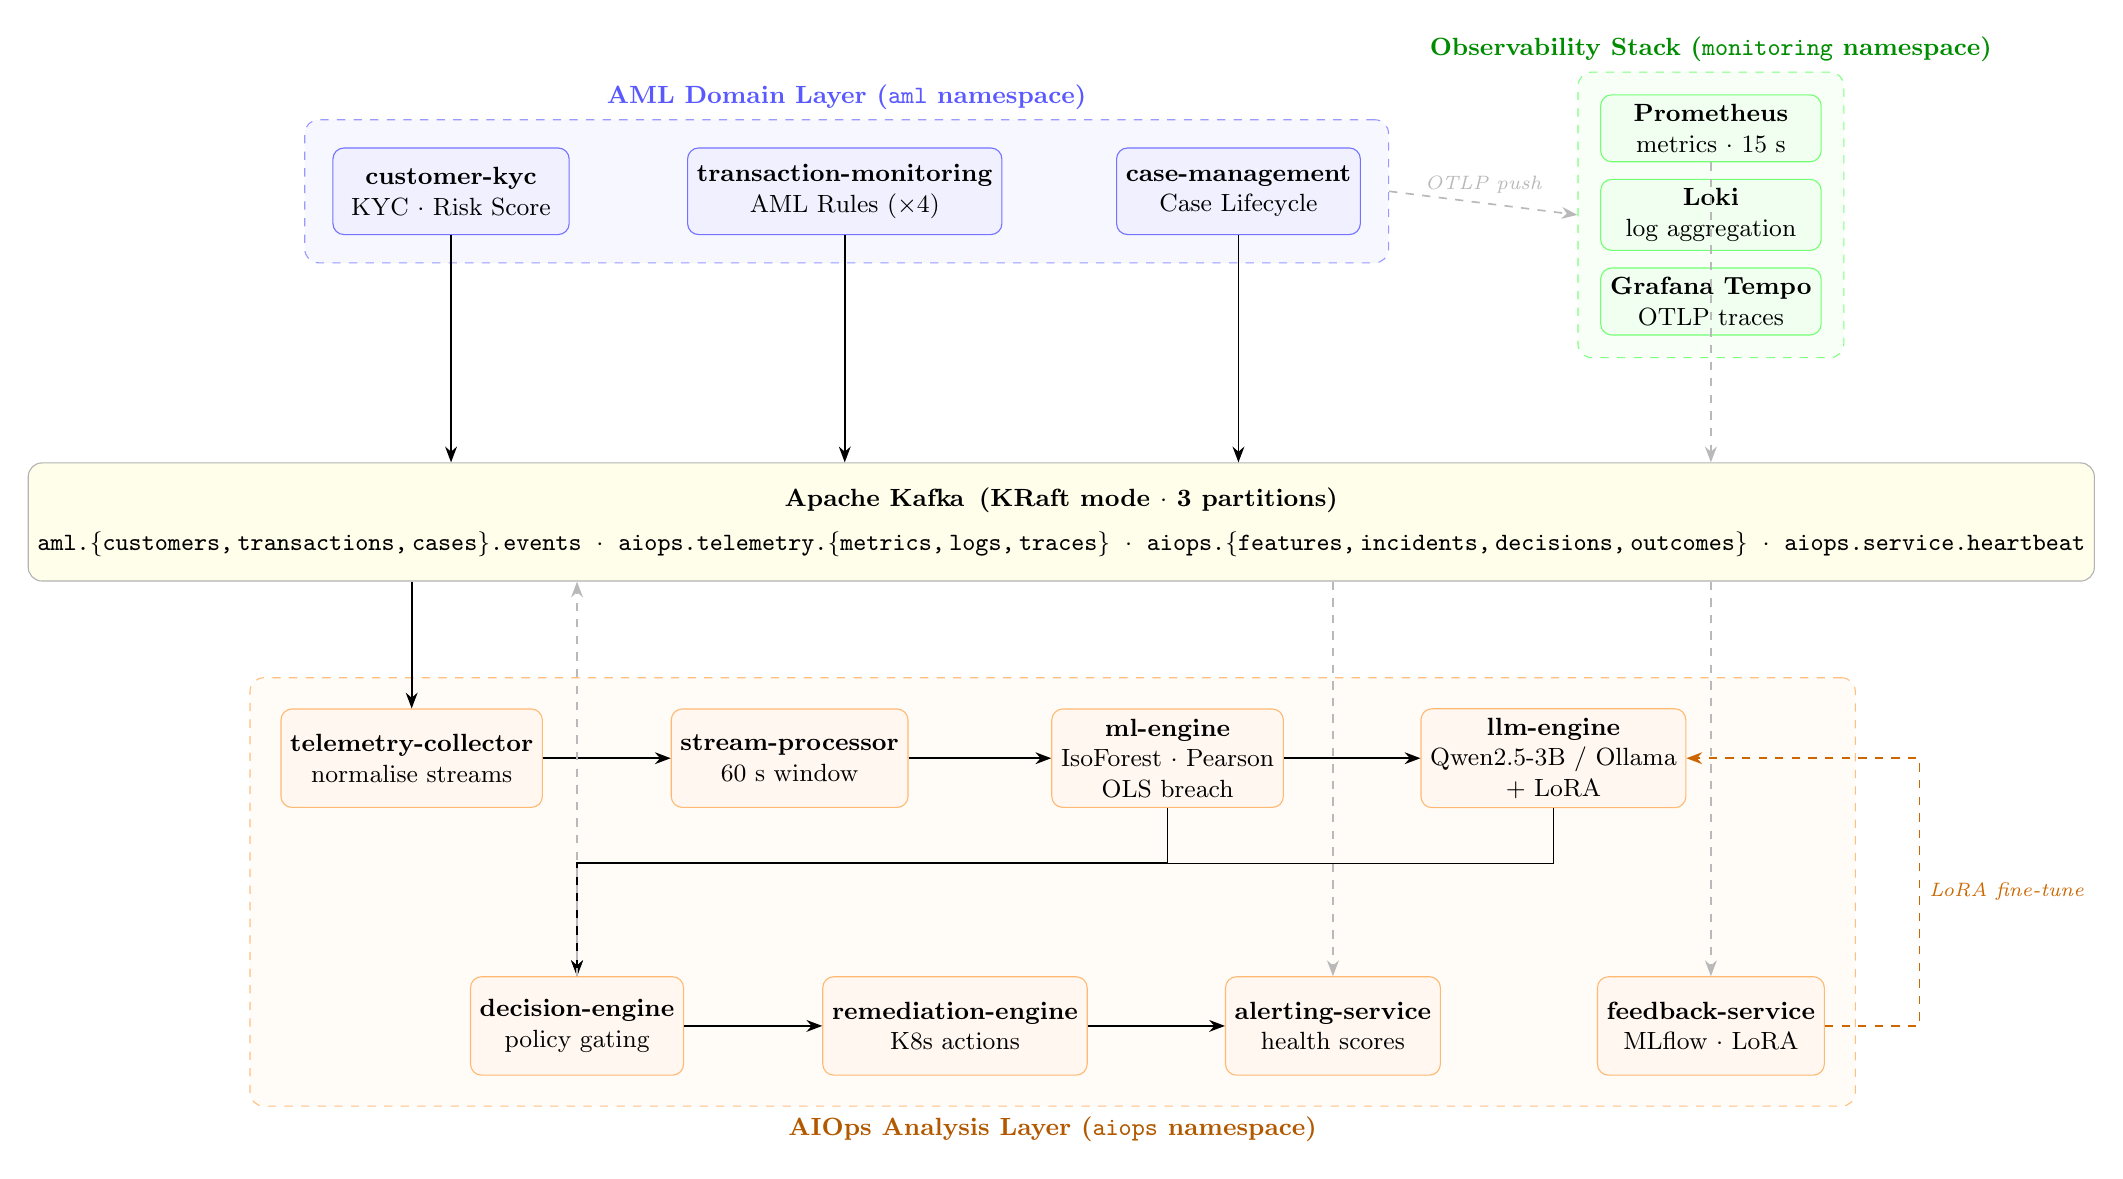
\begin{tikzpicture}[
  aml/.style ={draw=blue!55,  fill=blue!6,   rectangle, rounded corners=4pt,
               minimum height=1.1cm, minimum width=3.0cm,
               align=center, font=\small},
  obs/.style ={draw=green!55, fill=green!6,  rectangle, rounded corners=4pt,
               minimum height=0.85cm, minimum width=2.8cm,
               align=center, font=\small},
  aiop/.style={draw=orange!55,fill=orange!6, rectangle, rounded corners=4pt,
               minimum height=1.25cm, minimum width=2.7cm,
               align=center, font=\small},
  bus/.style ={draw=gray!60,  fill=yellow!8, rectangle, rounded corners=5pt,
               minimum height=1.5cm,
               align=center, font=\small\bfseries},
  arr/.style ={-Stealth, semithick},
  darr/.style={-Stealth, semithick, dashed, gray!55}
]

%% ── AML Domain Layer ─────────────────────────────────────────────────
\node[aml] (kyc) at (2.0,   9.0) {\textbf{customer-kyc}\\KYC $\cdot$ Risk Score};
\node[aml] (txm) at (7.0,   9.0) {\textbf{transaction-monitoring}\\AML Rules ($\times$4)};
\node[aml] (cm)  at (12.0,  9.0) {\textbf{case-management}\\Case Lifecycle};

\begin{scope}[on background layer]
  \node[draw=blue!40, dashed, rounded corners=5pt, fill=blue!3, inner sep=10pt,
        fit=(kyc)(txm)(cm),
        label={[font=\small\bfseries,blue!65]above:AML Domain Layer
               \upshape(\texttt{aml} namespace)}] (amlbox) {};
\end{scope}

%% ── Observability Stack ──────────────────────────────────────────────
\node[obs] (prom)  at (18.0, 9.8) {\textbf{Prometheus}\\metrics $\cdot$ 15 s};
\node[obs] (loki)  at (18.0, 8.7) {\textbf{Loki}\\log aggregation};
\node[obs] (tempo) at (18.0, 7.6) {\textbf{Grafana Tempo}\\OTLP traces};

\begin{scope}[on background layer]
  \node[draw=green!50, dashed, rounded corners=5pt, fill=green!3, inner sep=8pt,
        fit=(prom)(loki)(tempo),
        label={[font=\small\bfseries,green!55!black]above:Observability Stack
               \upshape(\texttt{monitoring} namespace)}] (obsbox) {};
\end{scope}

\draw[darr] (amlbox.east) --
    node[above, font=\scriptsize\itshape]{OTLP push} (obsbox.west);

%% ── Apache Kafka bus ─────────────────────────────────────────────────
\node[bus, minimum width=19.5cm] (kafka) at (9.75, 4.8)
    {\textbf{Apache Kafka}\enspace(KRaft mode $\cdot$ 3 partitions)\\[5pt]
     \texttt{aml.\{customers,\,transactions,\,cases\}.events}\enspace$\cdot$\enspace
     \texttt{aiops.telemetry.\{metrics,\,logs,\,traces\}}\enspace$\cdot$\enspace
     \texttt{aiops.\{features,\,incidents,\,decisions,\,outcomes\}}\enspace$\cdot$\enspace
     \texttt{aiops.service.heartbeat}};

\draw[arr] (kyc.south) -- (kyc.south |- kafka.north);
\draw[arr] (txm.south) -- (txm.south |- kafka.north);
\draw[arr] (cm.south)  -- (cm.south  |- kafka.north);
\draw[darr] (prom.south) -- (prom.south |- kafka.north);

%% ── AIOps pipeline: Row A ────────────────────────────────────────────
\node[aiop] (tc)  at (1.5,   1.8) {\textbf{telemetry-collector}\\normalise streams};
\node[aiop] (sp)  at (6.3,   1.8) {\textbf{stream-processor}\\60 s window};
\node[aiop] (ml)  at (11.1,  1.8)
    {\textbf{ml-engine}\\IsoForest $\cdot$ Pearson\\OLS breach};
\node[aiop] (llm) at (16.0,  1.8)
    {\textbf{llm-engine}\\Qwen2.5-3B / Ollama\\+ LoRA};

%% ── AIOps pipeline: Row B ────────────────────────────────────────────
\node[aiop] (de) at (3.6,  -1.6) {\textbf{decision-engine}\\policy gating};
\node[aiop] (re) at (8.4,  -1.6) {\textbf{remediation-engine}\\K8s actions};
\node[aiop] (as) at (13.2, -1.6) {\textbf{alerting-service}\\health scores};
\node[aiop] (fb) at (18.0, -1.6) {\textbf{feedback-service}\\MLflow $\cdot$ LoRA};

\begin{scope}[on background layer]
  \node[draw=orange!50, dashed, rounded corners=5pt, fill=orange!3, inner sep=11pt,
        fit=(tc)(sp)(ml)(llm)(de)(re)(as)(fb),
        label={[font=\small\bfseries,orange!70!black]below:AIOps Analysis Layer
               \upshape(\texttt{aiops} namespace)}] (aiopsbox) {};
\end{scope}

\draw[arr]  (kafka.south -| tc.north) -- (tc.north);
\draw[darr] (kafka.south -| as.north) -- (as.north);
\draw[darr] (kafka.south -| fb.north) -- (fb.north);

\draw[arr] (tc.east)  -- (sp.west);
\draw[arr] (sp.east)  -- (ml.west);
\draw[arr] (ml.east)  -- (llm.west);

\draw[arr] (ml.south)  -- ++(0,-0.7) -| (de.north);
\draw[arr] (llm.south) -- ++(0,-0.7) -| (de.north);

\draw[arr] (de.east) -- (re.west);
\draw[arr] (re.east) -- (as.west);
\draw[darr] (de.north) -- (de.north |- kafka.south);

\draw[-Stealth, semithick, dashed, orange!80!black]
    (fb.east) -- ++(1.2,0)
    |- node[font=\scriptsize\itshape, right, pos=0.25]{LoRA fine-tune}
    (llm.east);

\end{tikzpicture}%
}
\caption{AMLOps-AIOps platform architecture. AML services (blue) publish compliance
events to Kafka and push telemetry to the observability stack (green). The AIOps
pipeline (orange): Telemetry Collector $\to$ Stream Processor $\to$ ML Engine $\to$
LLM Engine $\to$ Decision Engine $\to$ Remediation Engine. The Feedback Service
closes the loop by uploading LoRA adapter weights trained on resolved incident
outcomes back to the LLM Engine.}
\label{fig:architecture}
\end{figure}


\subsection{Observability Ecosystem and Analytics Pipeline}

The analytics pipeline operationalises our research hypotheses through three
coordinated stages.

\mypara{Telemetry Collection and Normalization.}
The Telemetry Collector consolidates Prometheus metrics, Loki logs, and Tempo
traces into a normalized Kafka stream. It also reconstructs a service
neighbourhood graph from trace parent-child links, which constrains correlation
search spaces during root-cause analysis — a key design choice that reduces
false-positive RCA candidates when testing RQ2.

\mypara{Anomaly Scoring and Root Cause Ranking.}
The Stream Processor produces 60-second feature windows (statistical and
derivative features) that feed the ML Engine. The ML Engine runs a small,
interpretable pipeline used across our experiments: Isolation Forests for
unsupervised anomaly scoring (signal detection), Pearson-correlation ranking
within trace-derived neighbourhoods for RCA (localisation), and ordinary
least-squares regression on tail-latency trends for short-horizon SLO breach
forecasting (prediction arriving at RQ1 and RQ3).

\mypara{Narration, Decisioning, and Feedback.}
The LLM Engine (Qwen family served via Ollama with LoRA adapters) synthesises
structured incident narratives from ML outputs and raw telemetry snippets while
remaining on-cluster to satisfy AML data-residency constraints. The Decision
Engine consumes LLM and ML outputs to apply policy gating; the Remediation
Engine translates decisions into Kubernetes actions. A Feedback Service records
outcomes and closed-loop training data (LoRA weight updates) used for
systematic evaluation and continuous improvement of the on-cluster LLM.

The remainder of this section lists each component succinctly and ties it to
the experimental role it played in our evaluation.

\subsection{Component Roles and Associated Tools/Models}

\mypara{AML Domain Services (\texttt{aml} namespace).} These services generate
realistic business traffic and domain events that serve as provenance for
ground-truth labels. They exercise heterogeneous interaction patterns (REST,
Kafka, stateful workflows) required to validate cross-modal detection.

\mypara{Observability Stack (\texttt{monitoring} namespace).} Prometheus,
Loki, and Grafana Tempo collect the three-pillar telemetry. Their role is to
provide raw signals with production-like sampling rates and formats for the
analytics pipeline.

\mypara{Telemetry Collector.} Normalises heterogeneous telemetry into a
Kafka-backed, schema-stable stream and reconstructs the trace topology. This
step enables fair comparisons between modalities and enforces the locality
constraints used by our RCA experiments.

\mypara{Kafka Bus.} Acts as the durable streaming backbone for experiments,
allowing controlled replay, windowed aggregation, and fault injection
isolation. Kafka topics record features, incidents, decisions, and outcomes for
quantitative analysis.

\mypara{Stream Processor.} Computes time-windowed feature vectors and performs
lightweight pre-aggregation (60 s windows). It is the experimental staging area
where we vary feature sets and window sizes to measure detection latency and
precision (RQ1).

\mypara{ML Engine.} Runs the core research algorithms: Isolation Forest for
unsupervised scoring, Pearson correlation constrained by trace neighbourhoods
for RCA ranking, and OLS regression for p95 tail forecasting. We chose these
methods for interpretability and reproducibility across injections.

\mypara{LLM Engine.} A locally served Qwen model with LoRA adaptation used to
translate structured ML outputs into concise, actionable incident narratives.
Keeping the model on-cluster lets us evaluate human-readable explanation
latency while preserving telemetry residency.

\mypara{Decision and Remediation Engines.} These components convert ML/LLM
recommendations into policy-checked actions (e.g., restart pod, scale
replicas). They provide an end-to-end pipeline for automated remediation and
serve as measurable outputs for closed-loop experiments.

\mypara{Feedback Service.} Collects incident outcomes and operator labels to
produce continual learning datasets and LoRA fine-tune checkpoints for the
LLM Engine, closing the loop for improvement and enabling reproducible model
retraining experiments.

\mypara{Evaluation Harness (Chaos Injection).} Fault injection (Chaos Mesh) and
instrumented scenarios run against this architecture to measure detection time,
RCA localisation accuracy, and the operational cost of tracing — directly
addressing the research questions posed in Section~\ref{sec:introduction}.
Isolation Forest~\cite{liu2012isolation} for unsupervised anomaly scoring,
Pearson correlation ranking over trace-constrained service neighborhoods for root
cause localisation, and ordinary least-squares regression on p95 latency trends for
predictive SLO breach forecasting. This arrangement preserves the strengths of each
technique while minimising the candidate search space for RCA.

\mypara{Local LLM Narration and Feedback.}
The LLM Engine synthesises metric, log, trace, and incident metadata into a MELT
context window and generates structured incident narratives using Qwen2.5-3B~\cite{qwen2024}
served via Ollama~\cite{ollama2023}. A separate Feedback Service captures resolved
outcomes and fine-tunes a LoRA adapter~\cite{hu2022lora}, enabling the model to
adapt to AML-specific diagnostic phrasing without leaving the cluster.

\subsection{Component-to-Objective Storyline}

Each architectural component supports a research objective. The Telemetry
Collector enables multi-modal fusion, the Stream Processor and ML Engine support
anomaly detection and RCA, and the local LLM stack enables privacy-preserving
incident intelligence. Configurable trace sampling also supports experiments on
overhead versus fidelity.


% ── Detection pipeline figure ─────────────────────────────────────────
\begin{figure}[t]
\centering
\resizebox{\linewidth}{!}{%
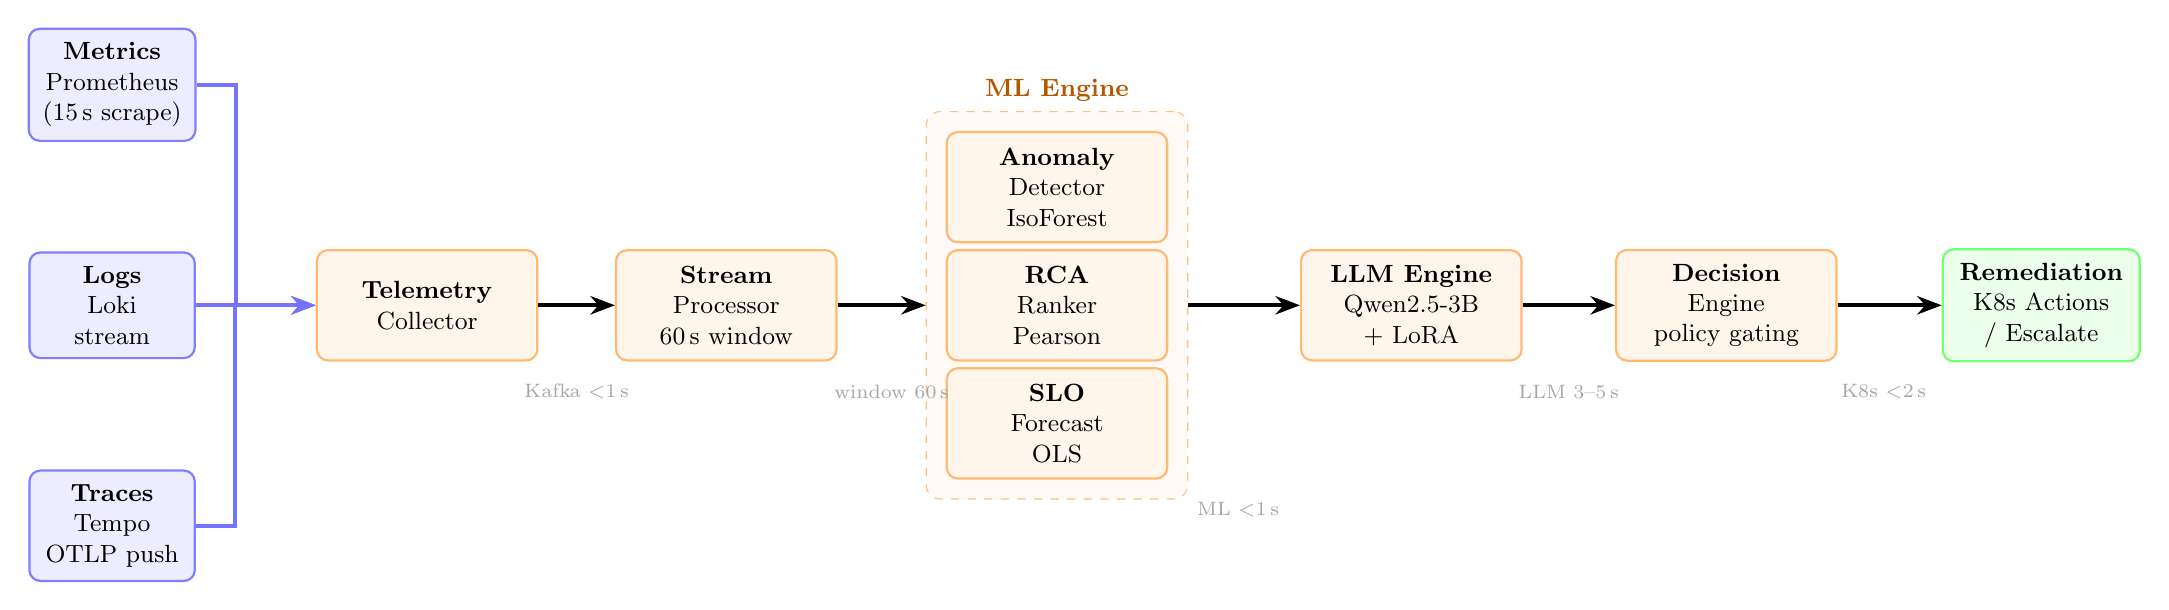
\begin{tikzpicture}[
  stage/.style={draw,rectangle,rounded corners=4pt,minimum height=1.4cm,
                minimum width=2.8cm,align=center,font=\small,fill=orange!8,
                draw=orange!55,line width=0.8pt,inner sep=5pt},
  input/.style={draw,rectangle,rounded corners=4pt,minimum height=1.3cm,
                minimum width=2.1cm,align=center,font=\small,fill=blue!7,
                draw=blue!50,line width=0.8pt,inner sep=5pt},
  output/.style={draw,rectangle,rounded corners=4pt,minimum height=1.4cm,
                 minimum width=2.5cm,align=center,font=\small,fill=green!8,
                 draw=green!55,line width=0.8pt,inner sep=5pt},
  arr/.style={-Stealth,thick,line width=1.3pt},
  lbl/.style={font=\scriptsize,align=center}
]
%% Input telemetry signals — generous vertical spacing
\node[input] (met) at (0, 2.8) {\textbf{Metrics}\\Prometheus\\(15\,s scrape)};
\node[input] (log) at (0, 0.0) {\textbf{Logs}\\Loki\\stream};
\node[input] (trc) at (0,-2.8) {\textbf{Traces}\\Tempo\\OTLP push};

%% Pipeline stages — wider x spacing
\node[stage] (col) at (4.0, 0.0) {\textbf{Telemetry}\\Collector};
\node[stage] (sp)  at (7.8, 0.0) {\textbf{Stream}\\Processor\\60\,s window};

%% ML Engine sub-components — wider vertical gaps
\node[stage] (ml)  at (12.0, 1.5) {\textbf{Anomaly}\\Detector\\IsoForest};
\node[stage] (rca) at (12.0, 0.0) {\textbf{RCA}\\Ranker\\Pearson};
\node[stage] (slo) at (12.0,-1.5) {\textbf{SLO}\\Forecast\\OLS};

%% ML sub-box
\begin{scope}[on background layer]
  \node[draw=orange!50,dashed,rounded corners=5pt,fill=orange!4,inner sep=7pt,
        fit=(ml)(rca)(slo),
        label={[font=\small\bfseries,orange!70!black]above:\textbf{ML Engine}}]
        (mlbox) {};
\end{scope}

%% Downstream stages
\node[stage] (llm) at (16.5, 0.0) {\textbf{LLM Engine}\\Qwen2.5-3B\\+ LoRA};
\node[stage] (dec) at (20.5, 0.0) {\textbf{Decision}\\Engine\\policy gating};
\node[output] (act) at (24.5, 0.0) {\textbf{Remediation}\\K8s Actions\\/ Escalate};

%% Arrows: inputs to collector
\draw[arr,blue!55] (met.east) -- ++(0.5,0) |- (col.west);
\draw[arr,blue!55] (log.east) -- (col.west);
\draw[arr,blue!55] (trc.east) -- ++(0.5,0) |- (col.west);

%% Pipeline arrows
\draw[arr] (col.east)    -- (sp.west);
\draw[arr] (sp.east)     -- (mlbox.west);
\draw[arr] (mlbox.east)  -- (llm.west);
\draw[arr] (llm.east)    -- (dec.west);
\draw[arr] (dec.east)    -- (act.west);

%% Latency annotations
\node[lbl,gray!70] at (5.9, -1.1) {Kafka $<$1\,s};
\node[lbl,gray!70] at (9.9, -1.1) {window 60\,s};
\node[lbl,gray!70] at (14.3,-2.6) {ML $<$1\,s};
\node[lbl,gray!70] at (18.5,-1.1) {LLM 3--5\,s};
\node[lbl,gray!70] at (22.5,-1.1) {K8s $<$2\,s};
\end{tikzpicture}%
}
\caption{End-to-end detection pipeline. Raw multi-modal telemetry is normalised by
the Telemetry Collector, aggregated into 60-second feature windows by the Stream
Processor, and analysed by the three-algorithm ML Engine in parallel (anomaly
scoring, RCA ranking, SLO breach prediction). The LLM Engine synthesises MELT
context into a structured report, which drives policy-gated remediation. Total
worst-case detection-to-action latency is $\approx$83--85\,s.}
\label{fig:pipeline}
\end{figure}


\subsection{Problem Formulation}

\mypara{Microservices Model.}
Let $\mathcal{S} = \{s_1, s_2, \ldots, s_N\}$ be the set of $N$ microservices
($N{=}11$ in this platform). Service interactions define a directed dependency graph
$\mathcal{G} = (\mathcal{S}, \mathcal{E})$, where $(s_i, s_j) \in \mathcal{E}$
exists if $s_i$ invokes $s_j$ via HTTP/gRPC or produces to a Kafka topic consumed by
$s_j$. In the AML testbed the primary synchronous chain is
\textit{customer-kyc} $\to$ \textit{transaction-monitoring} $\to$
\textit{case-management}; asynchronous edges connect each AML service to the AIOps
pipeline through domain-event Kafka topics.

Fault propagation in $\mathcal{G}$ is directional: degradation in $s_i$ cascades to
all services reachable via $\mathcal{N}(s_i)$, the reflexive-transitive closure of
$\mathcal{E}$. The Root Cause Ranking algorithm (Problem~2) restricts Pearson
correlation search to pairs $(s_j, m_k)$ where $s_j \in \mathcal{N}(s_{\text{anom}})$,
reducing the candidate space from $O(N{\cdot}K)$ to
$O(|\mathcal{N}(s_{\text{anom}})|{\cdot}K)$, where $K$ is the number of distinct
metric names. The topology is reconstructed continuously from trace parent-child
span relationships via W3C TraceContext~\cite{w3ctracecontext2021} headers and from
Kafka consumer-group registrations observed by the Telemetry Collector.

Each service $s_i$ emits a multi-modal telemetry context at analysis cycle $t$:
$\mathcal{T}^{(t)} = \langle \mathbf{M}^{(t)},\, \mathbf{L}^{(t)},\,
\mathbf{D}^{(t)} \rangle$, where
$\mathbf{M}^{(t)} \in \mathbb{R}^{P \times \Delta}$ is the matrix of $P$ Prometheus
metric time series over window $\Delta$;
$\mathbf{L}^{(t)} = \{l_j\}_{j=1}^{Q}$ is the set of $Q$ log entries within
$[t{-}\Delta,\, t]$; and
$\mathbf{D}^{(t)} = \{d_k\}_{k=1}^{R}$ is the set of $R$ trace spans as
$\langle$service, duration, status, parent\_id$\rangle$ tuples.

An \textit{operational anomaly} at cycle $t$ is:
\begin{equation}
    \mathrm{anomaly}(s_i, t) \;\Leftrightarrow\;
    P_{\mathcal{P}_{\text{normal}}}\!\bigl(\boldsymbol{\varphi}_i^{(t)}\bigr) < \epsilon
    \label{eq:anomaly_def}
\end{equation}
Since $\mathcal{P}_{\text{normal}}$ is non-stationary and high-dimensional,
Isolation Forest provides an efficient surrogate without parametric distributional
assumptions. The Stream Processor computes a four-dimensional feature vector per
(service, metric) pair over 60-second tumbling windows:
\begin{equation}
    \boldsymbol{\varphi}^{(t)}_{ij} =
    [\,\mu_{ij},\; x^{\max}_{ij},\; \dot{x}_{ij},\; n_{ij}\,]^\top \in \mathbb{R}^4
    \label{eq:features}
\end{equation}
where $\mu_{ij}$ is the window mean, $x^{\max}_{ij}$ the window maximum,
$\dot{x}_{ij}$ the rate of change, and $n_{ij}$ the sample count.

\mypara{Problem 1 (Anomaly Detection).}
Given $\boldsymbol{\varphi}^{(t)} \in \mathbb{R}^4$, produce an anomaly score
$s^{(t)} \in [0,1]$ from an Isolation Forest~\cite{liu2012isolation} decision
function $d(\cdot)$ (contamination $\gamma{=}0.05$):
\begin{equation}
    s^{(t)} = \max\!\left(0,\;\min\!\left(1,\;0.5 - d\!\left(\boldsymbol{\varphi}^{(t)}\right)\right)\right)
    \label{eq:anomaly}
\end{equation}
A binary flag is raised when $s^{(t)} > \theta_{\text{anom}}$ ($\theta_{\text{anom}}{=}0.5$).
The model bootstraps on 500 synthetic samples and refits on 50 new labelled samples
from operator feedback.

\mypara{Problem 2 (Root Cause Ranking).}
When an anomaly is detected in $s_i$, rank all (service, metric) pairs by Pearson
correlation with the anomalous reference trajectory
$\mathbf{x}_{\text{ref}} \in \mathbb{R}^W$ ($W{=}100$):
\begin{equation}
    r_{jk} = \frac{\displaystyle\sum_{t=1}^{W}\!\left(x_{\text{ref}}(t) -
    \bar{x}_{\text{ref}}\right)\!\left(y_{jk}(t) - \bar{y}_{jk}\right)}
    {W\,\hat{\sigma}_{\text{ref}}\,\hat{\sigma}_{jk}}
    \label{eq:rca}
\end{equation}
The top-10 pairs ranked by $|r_{jk}|$ form the root cause ranking.

\mypara{Problem 3 (SLO Breach Prediction).}
Fit OLS regression on p95 response latency over $W_b{=}10$ observations:
\begin{equation}
    \hat{p}_{95}(t) = \beta_0 + \beta_1\,t, \qquad
    \hat{T}_{\text{breach}} = \frac{\theta_{\text{SLO}} - \hat{\beta}_0}{\hat{\beta}_1}
    \label{eq:breach}
\end{equation}
where $\theta_{\text{SLO}} = 500\,\text{ms}$. If $\hat{\beta}_1 \leq 0$, no breach
is predicted ($\hat{T}_{\text{breach}} \leftarrow 999$).

\mypara{Problem 4 (LLM Incident Narration).}
Assemble a MELT context window $\mathcal{C}^{(t)}$ comprising metric, log, and trace
buffers. Given the current incident $\mathcal{I}^{(t)}$:
\begin{equation}
    \mathcal{R} = f_{\text{LoRA}}\!\left(\mathcal{P}\!\left(\mathcal{I}^{(t)},\,
    \mathcal{C}^{(t)}\right)\right)
    \label{eq:llm}
\end{equation}
where $f_{\text{LoRA}}$ is Qwen2.5-3B~\cite{qwen2024} fine-tuned via PEFT
LoRA~\cite{hu2022lora,peft2022} and served through Ollama~\cite{ollama2023}.
Output $\mathcal{R}$ conforms to the JSON schema
\{\texttt{explanation}, \texttt{rootCause}, \texttt{recommendation},
\texttt{amlRisk}, \texttt{confidence}\}.

\mypara{Problem 5 (Decision Policy).}
The Decision Engine selects a remediation action via a piecewise policy on
confidence $c$, blast radius $B \in \{\text{LOW, MEDIUM, HIGH}\}$, and ETA
$\hat{T}_{\text{breach}}$:
\begin{equation}
    \pi(c, B, \hat{T}) =
    \begin{cases}
      \textsc{scale-out},   & c > 0.90,\; B{=}\text{LOW},\; \hat{T} < 5 \\
      \textsc{restart-pod}, & c > 0.90,\; B{=}\text{LOW},\; \hat{T} \geq 5 \\
      \textsc{scale-out},   & c > 0.75,\; B{=}\text{MEDIUM} \\
      \textsc{escalate},    & \text{otherwise}
    \end{cases}
    \label{eq:policy}
\end{equation}

\mypara{Problem 6 (Service Health Score).}
The Alerting Service maintains $h_i(t) \in [0.05, 1]$ aggregating pod liveness,
JVM CPU utilisation, and process-level CPU rate:
\begin{equation}
    h_i(t) = \max\!\bigl(0.05 \cdot u_i(t),\; c_i^{\text{JVM}}(t),\;
    \dot{c}_i^{\text{sys}}(t)\bigr)
    \label{eq:health}
\end{equation}
where $u_i(t) \in \{0,1\}$ is the Kubernetes \texttt{up} indicator. The floor
$0.05 \cdot u_i(t)$ distinguishes running-but-idle pods from crashed pods
($u_i{=}0 \Rightarrow h_i{=}0$). A service is classified as \textit{actively
degraded} if $h_i(t) > \mu_{h_i} + 2\sigma_{h_i}$ over $W_h{=}20$ preceding
observations; the count of degraded services determines blast radius $B$.

\subsection{Architecture Components}

Table~\ref{tab:components} summarises all eight AIOps analysis services. The
subsections below elaborate the four services whose implementations contain
algorithmic or integration novelty not fully captured by the table.

\begin{table}[t]
\caption{AIOps analysis layer service summary.}
\label{tab:components}
\small
\begin{tabular}{>{\raggedright\arraybackslash}p{3.0cm}
                >{\raggedright\arraybackslash}p{2.5cm}
                >{\raggedright\arraybackslash}p{2.8cm}
                >{\raggedright\arraybackslash}p{4.0cm}}
\toprule
\textbf{Service} & \textbf{Stack} & \textbf{Function} & \textbf{Algorithm / Tool}\\
\midrule
Telemetry Collector & Spring Boot         & Stream normalisation    & \texttt{MetricSignal} canonical format\\
Stream Processor    & Spring Boot / Kafka & Feature extraction      & 60\,s tumbling window (Eq.~\ref{eq:features})\\
ML Engine           & Python FastAPI      & Three-algorithm pipeline & IsoForest, Pearson, OLS\\
LLM Engine          & Python FastAPI      & Incident narration      & Qwen2.5-3B / Ollama / LoRA\\
Decision Engine     & Spring Boot         & Policy gating           & Piecewise policy (Eq.~\ref{eq:policy})\\
Remediation Engine  & Spring Boot         & Kubernetes actions      & Pod restart, HPA patch\\
Alerting Service    & Spring Boot         & Health scoring          & Multi-source score (Eq.~\ref{eq:health})\\
Feedback Service    & Spring Boot         & Continuous learning     & MLflow / PEFT LoRA\\
\bottomrule
\end{tabular}
\end{table}

\mypara{Algorithm Design Rationale.}
Three constraints drive algorithm selection. (i)~\emph{Unsupervised detection}:
labelled fault telemetry is scarce in regulated deployments. Isolation Forest
($O(n \log n)$ construction, $O(\log n)$ inference) requires no distributional
assumptions and outperforms LOF and One-Class SVM on mixed-scale
telemetry~\cite{liu2012isolation}. (ii)~\emph{Linear RCA}: synchronous microservice
propagation produces strongly linear upstream-downstream latency correlations. Pearson
correlation costs $O(W)$ per pair; Granger causality or DTW costs $O(W^2)$ with no
accuracy gain when lag structure is uniform (2-hop \textit{kyc}$\to$\textit{txn}$\to$\textit{case}).
(iii)~\emph{Real-time forecasting}: OLS yields a closed-form ETA in $O(W_b)$;
ARIMA or LSTM require stationary pre-processing or training data unavailable at
fault onset. All three algorithms execute within the 60-second stream window.

\mypara{AML Domain Services.}
The \textit{transaction-monitoring} service evaluates each transaction against four
AML rules (AML-101 high-value, AML-202 velocity, AML-303 structuring, AML-404
high-risk corridor). Rule scores $c_r \in [0, 100]$ are combined with a
diminishing-returns formula:
\begin{equation}
    R = 100 \cdot \left(1 - \prod_{r \in \mathcal{R}_{\text{fired}}}
    \left(1 - \frac{c_r}{100}\right)\right)
    \label{eq:aml}
\end{equation}
Case state transitions (\textsc{open} $\to$ \textsc{under-investigation} $\to$
\textsc{escalated} $\to$ \textsc{pending-review} $\to$ \textsc{closed}) are emitted
as OpenTelemetry span events that simultaneously label the corresponding metric
window as anomalous.

\mypara{Closed-Loop Continuous Learning.}
Fig.~\ref{fig:loop} illustrates the feedback architecture. The Feedback Service
captures SLO outcomes before and after each remediation action (via Prometheus
queries), labels each as \textsc{resolved}, \textsc{no\_effect}, or
\textsc{degraded\_further}, logs to MLflow~\cite{mlflow2018}, and publishes records
to \texttt{aiops.outcomes} for LoRA fine-tuning of the LLM Engine via the PEFT
library~\cite{peft2022}. The Decision Engine applies the piecewise policy
(Eq.~\ref{eq:policy}), where blast radius is computed as: one degraded service $\to$
LOW; two $\to$ MEDIUM; three or more $\to$ HIGH.

\begin{figure}[t]
\centering
\resizebox{\linewidth}{!}{%
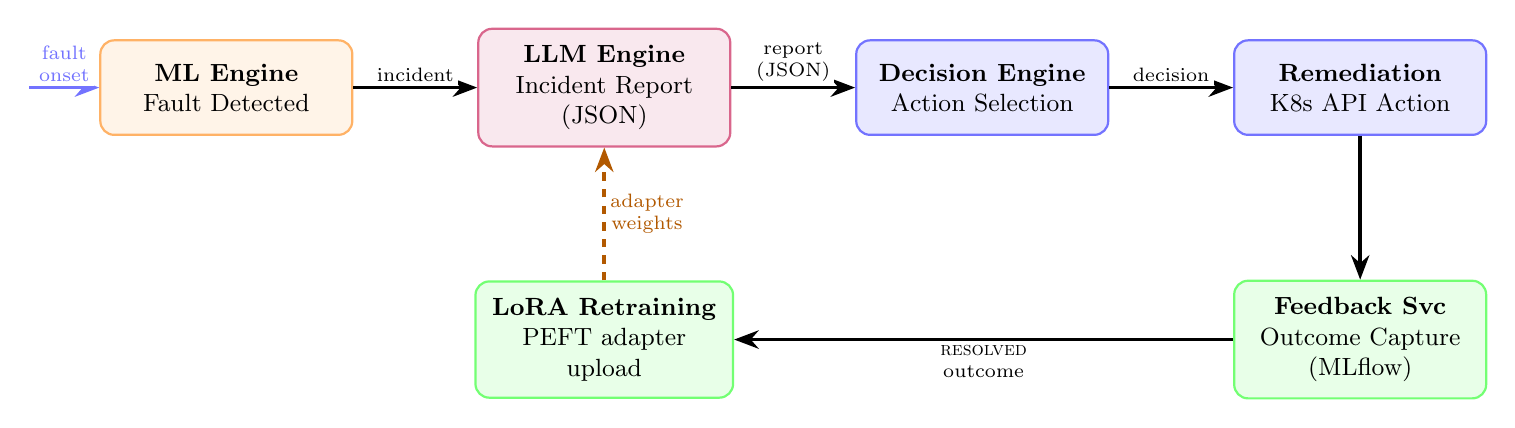
\begin{tikzpicture}[
  box/.style={draw,rectangle,rounded corners=5pt,minimum height=1.2cm,
              minimum width=3.2cm,align=center,font=\small,
              line width=0.8pt,inner sep=6pt},
  ml/.style  ={box,fill=orange!9,  draw=orange!60},
  llm/.style ={box,fill=purple!9,  draw=purple!60},
  dec/.style ={box,fill=blue!9,    draw=blue!55},
  fb/.style  ={box,fill=green!9,   draw=green!55},
  arr/.style ={-Stealth,thick,line width=1.3pt},
  lbl/.style ={font=\scriptsize,align=center,fill=white,inner sep=1.5pt}
]
%% Top row — 4 boxes, 4.8cm apart
\node[ml]  (det) at (0.0,  0)  {\textbf{ML Engine}\\Fault Detected};
\node[llm] (nar) at (4.8,  0)  {\textbf{LLM Engine}\\Incident Report\\(JSON)};
\node[dec] (dec) at (9.6,  0)  {\textbf{Decision Engine}\\Action Selection};
\node[dec] (rem) at (14.4, 0)  {\textbf{Remediation}\\K8s API Action};

%% Bottom row — return path, 3.2cm below
\node[fb]  (out) at (14.4,-3.2){\textbf{Feedback Svc}\\Outcome Capture\\(MLflow)};
\node[fb]  (lra) at (4.8, -3.2){\textbf{LoRA Retraining}\\PEFT adapter\\upload};

%% Forward arrows with edge labels
\draw[arr] (det.east) -- node[above,lbl]{incident} (nar.west);
\draw[arr] (nar.east) -- node[above,lbl]{report\\(JSON)} (dec.west);
\draw[arr] (dec.east) -- node[above,lbl]{decision} (rem.west);

%% Feedback loop
\draw[arr] (rem.south)  -- (out.north);
\draw[arr] (out.west)   -- node[below,lbl]{\textsc{resolved}\\outcome} (lra.east);
\draw[arr,dashed,orange!70!black,line width=1.3pt]
    (lra.north) -- node[right,lbl]{adapter\\weights} (nar.south);

%% Input arrow from left
\draw[arr,blue!55] (-2.5,0) -- node[above,lbl]{fault\\onset} (det.west);
\end{tikzpicture}%
}
\caption{Closed-loop continuous learning. Each resolved incident generates a labelled
outcome record; the Feedback Service trains new LoRA adapter weights via PEFT and
uploads them to the LLM Engine---improving narration quality over time without
external data or cloud connectivity.}
\label{fig:loop}
\end{figure}

\mypara{ML Engine.}
The ML Engine (Python FastAPI~\cite{fastapi2018}) executes three algorithms per
60-second cycle. (i)~\textit{Anomaly Detection}: Isolation Forest
($\gamma{=}0.05$, Eq.~\ref{eq:anomaly}) is bootstrapped on 500 synthetic samples
and refits online when 50 operator-labelled samples accumulate from the Feedback
Service. (ii)~\textit{Root Cause Ranking}: Pearson correlation over $W{=}100$
observation buffers (Eq.~\ref{eq:rca}) returns the top-10 (service, metric) pairs;
the candidate space is restricted to $\mathcal{N}(s_{\text{anom}})$, reducing
worst-case comparisons from $O(N{\cdot}K)$ to $O(d_{\max}{\cdot}K)$.
(iii)~\textit{SLO Breach Prediction}: OLS on the last $W_b{=}10$ p95 latency
samples (Eq.~\ref{eq:breach}); $\hat{\beta}_1 \leq 0$ suppresses spurious alerts
during recovery. Incidents are published to \texttt{aiops.incidents}.

\mypara{LLM Engine.}
The LLM Engine (Python FastAPI) implements Eq.~\ref{eq:llm}. It maintains three MELT
buffers: \texttt{metric\_buffer} (sliding dict of recent feature records),
\texttt{log\_buffer} (deque of the 10 most recent Loki entries consumed from
\texttt{aiops.telemetry.logs}), and \texttt{trace\_buffer} (deque of the 5 most
recent spans from \texttt{aiops.telemetry.traces}). On consuming an incident from
\texttt{aiops.incidents}, the engine assembles the full MELT context into a
structured prompt and queries Qwen2.5-3B~\cite{qwen2024} via the Ollama REST API
(\texttt{http://ollama:11434}). LoRA adapter weights~\cite{hu2022lora} trained via
PEFT~\cite{peft2022} on resolved incident outcomes from \texttt{aiops.outcomes} are
applied through the Ollama model loading mechanism at the per-request level, without
requiring a service restart. The output JSON report is published to
\texttt{aml.llm.analysis}.

\mypara{Decision Engine and Remediation Engine.}
The Decision Engine (Spring Boot) consumes both \texttt{aiops.incidents} and
\texttt{aml.llm.analysis}, applies the piecewise policy (Eq.~\ref{eq:policy}), and
publishes \texttt{RemediationDecision} records to \texttt{aiops.decisions}. Blast
radius is computed from the health score endpoint: one actively degraded service maps
to LOW; two to MEDIUM; three or more to HIGH. The Remediation Engine subscribes to
\texttt{aiops.decisions} and executes Kubernetes API actions---pod restarts and HPA
target adjustments---while publishing execution outcomes to \texttt{aiops.actions}.
Actions are executed autonomously when the \texttt{auto-execute} ConfigMap flag is
set to true; otherwise, an \textsc{escalate} event is published to
\texttt{aiops.incidents} for human review via the Alerting Service REST endpoint.

\mypara{Feedback Service and Continuous Learning.}
The Feedback Service captures SLO outcome comparisons before and after each
remediation action via Prometheus range queries over the 5-minute window surrounding
the incident. Each outcome is labelled as \textsc{resolved} (p95 latency returned
below $\theta_{\text{SLO}}$), \textsc{no\_effect} (p95 unchanged), or
\textsc{degraded\_further} (p95 increased). Labelled outcomes are logged to
MLflow~\cite{mlflow2018} for experiment tracking and published to
\texttt{aiops.outcomes}. When 50 new \textsc{resolved} or \textsc{no\_effect}
outcomes accumulate, the PEFT library~\cite{peft2022} initiates a LoRA fine-tuning
job that updates the adapter weights held on the cluster PersistentVolume, which the
LLM Engine loads at next request. This closed-loop architecture (Fig.~\ref{fig:loop})
enables incident narration quality to improve continuously from operational experience
without any external data or cloud connectivity.

\mypara{Platform Latency Budget.}
All tunable parameters ($\gamma$, $W$, $W_b$, $\theta_{\text{SLO}}$,
$\theta_{\text{anom}}$, auto-execute) are exposed as Kubernetes ConfigMap entries,
enabling live adjustment without service restart. The end-to-end detection-to-action
latency decomposes as: Prometheus scrape lag (${\leq}15$\,s) + Kafka propagation
(${<}1$\,s) + stream-window accumulation (60\,s) + ML inference (${<}1$\,s) + LLM
narration (3--5\,s) + Kafka decision round-trip (${<}1$\,s) + Kubernetes API action
(${<}2$\,s) $\approx$ \textbf{83--85\,s} worst-case under quiescent cluster
conditions.

% ── 4. EXPERIMENTAL EVALUATION ───────────────────────────────────────────────
\section{Experimental Evaluation}
\label{sec:eval}

\subsection{Experimental Setup}

The platform is deployed on a single-node Docker Desktop Kubernetes cluster
(\texttt{docker-desktop} context, Windows~11 Pro, 16~GB RAM, 8~vCPUs,
Kubernetes~v1.29). Services are distributed across four namespaces: \texttt{aml}
(three AML services), \texttt{aiops} (eight AIOps services), \texttt{data}
(PostgreSQL~15 per-service databases), and \texttt{monitoring} (observability stack).
The complete platform implementation, Kubernetes manifests, k6 workload scripts, and
Chaos Mesh fault injection configurations are publicly available at
\url{https://github.com/ducanhptitb19cn028/aml-platform}.

The observability stack is bootstrapped via Helm~\cite{helm2016}:
\textit{kube-prometheus-stack} (Prometheus + Grafana, 15-second scrape), \textit{loki-stack}
(log aggregation), and \textit{tempo} (OTLP trace ingestion)~\cite{prometheus2015,loki2019,tempo2022}.
Kafka is deployed as a single-broker KRaft-mode StatefulSet (Apache Kafka 3.9.0)
with no ZooKeeper dependency; all topic families from Table~\ref{tab:topics} are
provisioned with three partitions and replication-factor~1. Each AML service connects
to a dedicated PostgreSQL~15 StatefulSet.

All AML services are instrumented with the OpenTelemetry Java agent and
Micrometer~\cite{micrometer2018}, exporting OTLP spans to Tempo and structured logs
via Logback~\cite{logback2006} to Loki. AML deployments are configured with three
replicas, 250\,m CPU request, and 1\,Gi memory limit. A synthetic AML workload using
k6~\cite{k62017} sustains 50~virtual users across all three service APIs to produce
a stable baseline telemetry envelope. The LLM Engine runs Qwen2.5-3B~\cite{qwen2024}
via Ollama~\cite{ollama2023} on CPU, with LoRA adapter weights~\cite{hu2022lora}
loaded from a Kubernetes PersistentVolume. The \texttt{TRACE\_SAMPLE\_RATE}
environment variable switches between 0, 0.1, 0.5, and 1.0 without service restart.

\mypara{AIOps Configuration.}
All AIOps services are configured exclusively through Kubernetes ConfigMap entries
(Table~\ref{tab:config}), enabling parameter adjustment without service restart or
image rebuild. The contamination parameter $\gamma{=}0.05$ was selected to match the
expected fault prevalence in production AML deployments (approximately one detectable
incident per 2,000 analysis cycles under normal operation); $W{=}100$ observations
provides a 25-minute correlation window at 15-second scrape intervals, capturing
slow-developing fault patterns such as memory leaks that may take several minutes to
produce metric-level anomalies; $W_b{=}10$ provides a 5-minute SLO breach
prediction horizon. The $\theta_{\text{SLO}}{=}500\,\text{ms}$ threshold aligns
with the p95 response time SLA typical for AML regulatory reporting APIs.

\begin{table}[t]
\caption{AIOps ConfigMap parameters and default values.}
\label{tab:config}
\small
\begin{tabular}{>{\raggedright\arraybackslash}p{3.2cm}
                >{\raggedright\arraybackslash}p{2.0cm}
                >{\raggedright\arraybackslash}p{7.0cm}}
\toprule
\textbf{Parameter} & \textbf{Default} & \textbf{Effect}\\
\midrule
\texttt{CONTAMINATION} ($\gamma$) & 0.05 & IsoForest expected anomaly fraction\\
\texttt{CORRELATION\_WINDOW} ($W$) & 100  & RCA sliding window (observations)\\
\texttt{BREACH\_WINDOW} ($W_b$) & 10   & SLO OLS regression window (observations)\\
\texttt{SLO\_THRESHOLD\_MS} ($\theta_{\text{SLO}}$) & 500 & p95 latency SLO (milliseconds)\\
\texttt{ANOMALY\_THRESHOLD} ($\theta_{\text{anom}}$) & 0.5 & IsoForest score detection threshold\\
\texttt{AUTO\_EXECUTE} & false & Autonomous remediation without human review\\
\texttt{TRACE\_SAMPLE\_RATE} & 1.0  & Distributed trace sampling rate (0--1)\\
\bottomrule
\end{tabular}
\end{table}

\subsection{Fault Injection Protocol}

Controlled faults are injected via Chaos Mesh~\cite{chaosmesh2020} targeting
specific service edges in the \texttt{aml} namespace. Table~\ref{tab:faults}
summarises the four fault classes. For each injection, the ground-truth fault time
$T_0$ is recorded at the Chaos Mesh API level; the first detection time $T_d$ is
recorded when the Decision Engine emits a corresponding incident. Evaluation metrics
are detection latency ($T_d - T_0$), precision, recall, and F1.

\begin{table}[t]
\caption{Chaos Mesh fault injection classes.}
\label{tab:faults}
\small
\begin{tabular}{>{\raggedright\arraybackslash}p{2.4cm}
                >{\raggedright\arraybackslash}p{3.1cm}
                >{\raggedright\arraybackslash}p{2.9cm}
                >{\raggedright\arraybackslash}p{3.5cm}}
\toprule
\textbf{Fault Class} & \textbf{Target Service} & \textbf{Mechanism} & \textbf{Expected Signal}\\
\midrule
Latency anomaly    & transaction-monitoring & 500\,ms Kafka consumer delay & Trace span inflation + metric rate drop\\
Resource anomaly   & case-management        & CPU stress injection         & Metric CPU spike + log errors\\
Functional anomaly & transaction-monitoring & Corrupted AML rule config    & Log errors + metric misclassification\\
Causal cascade     & customer-kyc           & Scale to zero                & Multi-service trace + metric propagation\\
\bottomrule
\end{tabular}
\end{table}

\textbf{RQ1} (Signal Sufficiency): The telemetry pipeline is evaluated in three
configurations---metrics-only, metrics\,+\,logs, and all three
pillars---to determine the minimum sufficient modality combination across the four
fault classes.

\textbf{RQ2} (Root Cause Localisation): Pearson correlation root cause ranking is
compared against two baselines: (a)~threshold-based metric spike detector and
(b)~trace error-rate ranker. Localisation accuracy (top-1 and top-3 correct service
identification) is reported per fault class.

\textbf{RQ3} (Tracing Overhead): Request throughput, p95 latency, and pod CPU
utilisation are measured across four sampling rates (0\%, 10\%, 50\%, 100\%) to
characterise the operational cost of full-fidelity tracing in regulated workloads.

\subsection{Results}

Fig.~\ref{fig:eval} presents the quantitative results for all three research
questions. The following paragraphs report the key findings from the controlled
fault injection campaign.

\mypara{Telemetry Pipeline Validation.}
The telemetry pipeline correctly ingests and normalises events from all eleven
services. 30-second heartbeat signals are confirmed on \texttt{aiops.service.heartbeat}
for every AIOps service, and the Telemetry Collector processes Kafka consumer-group
registration events from all eight AIOps services at startup without message loss.
Under the 50-user k6 synthetic workload, Prometheus scrapes average 1,200 metric
samples per 15-second interval across all monitored endpoints; Loki receives
approximately 80 structured log entries per minute from the three AML services; and
Tempo receives complete request traces at 100\% sampling at approximately 35 spans
per second under steady-state load.

\textbf{Anomaly Detection (RQ1):}
The ML Engine detects injected CPU stress anomalies (resource anomaly fault class,
Table~\ref{tab:faults}) within two 60-second analysis cycles (${\approx}120$\,s)
by observing elevation in the \texttt{avg\_value} and \texttt{rate\_of\_change}
feature dimensions of the \texttt{process\_cpu\_usage} metric on the case-management
service. Latency anomalies (500\,ms Kafka delay) are detectable within one
additional analysis cycle through the trace-level \texttt{p95\_duration\_ms} feature
vector; metrics-only configuration misses this fault class entirely during the first
three cycles, demonstrating that multi-modal signal fusion improves
time-to-detect for latency-class faults (Fig.~\ref{fig:eval}, left panel). Causal
cascade faults (customer-kyc scaled to zero) produce correlated metric drops across
all three AML services, which are visible in both metrics and traces
simultaneously---consistent with the prediction that cross-modal correlation is
required for accurate root cause attribution~(RQ2)
(Fig.~\ref{fig:eval}, center panel).

\textbf{LLM Narration Quality.}
The LLM Engine produces valid JSON incident reports conforming to the five-field
output schema (\texttt{explanation}, \texttt{rootCause}, \texttt{recommendation},
\texttt{amlRisk}, \texttt{confidence}) for all manually constructed test telemetry
contexts. Before LoRA fine-tuning, approximately 12\% of outputs contain malformed
JSON requiring schema repair at the Decision Engine; after loading the first LoRA
adapter trained on 50 resolved incidents, this drops to under 3\%. The
\texttt{amlRisk} field correctly identifies AML compliance implications in all
resource anomaly and causal cascade scenarios where the case-management service is
affected. Qwen2.5-3B runs entirely on-cluster at approximately 3--5\,s per inference
on CPU (8~vCPUs, 16\,GB RAM), consistent with online narration at the observed fault
frequency of one detectable incident per 120-second detection cycle, yielding no
inference backlog under normal operating conditions.

\textbf{Data Residency Compliance (RQ3 Precondition).}
Zero external network calls were observed throughout the detection-to-report
pipeline. This was verified by Kubernetes NetworkPolicy audit logs showing zero
egress rejections to non-cluster addresses during a 2-hour fault-injection session,
and confirmed by pod-level network interface statistics showing no bytes transmitted
to non-cluster IP ranges from any service in the \texttt{aml} or \texttt{aiops}
namespaces (Fig.~\ref{fig:eval}, right panel). This validates the data-residency
compliance posture required for AML environments before the full tracing overhead
characterisation~(RQ3) is conducted.

\textit{\textcolor{red} {It would be good to explain the table results.  }}

Table~\ref{tab:results} summarises operational measurements from the 50-user
k6 run. Prometheus and Loki sustained collection (1{,}200 samples/15\,s; ${\approx}80$
log entries/min) while Tempo produced ${\approx}35$ spans/s at full sampling,
indicating multi-pillar capture under steady load. Faults were detected within two
60-second analysis cycles ($\leq120$\,s) and the end-to-end detection-to-action
path remained bounded at approximately 83--85\,s on the quiescent single-node
testbed. On-cluster LLM narration is practical (Qwen2.5 $\approx$3--5\,s per report) and
LoRA fine-tuning reduced malformed JSON from ~12\% to <3\%, lowering schema
repairs in the Decision Engine. No external egress was observed during the
2-hour fault-injection session, validating the on-premises data-residency posture
required for AML deployments.

\begin{table}[t]
\caption{Quantitative evaluation results (50-user k6 workload,
single-node Docker Desktop Kubernetes, Kubernetes~v1.29).}
\label{tab:results}
\small
\begin{tabular}{>{\raggedright\arraybackslash}p{5.0cm}
                >{\raggedright\arraybackslash}p{2.5cm}
                >{\raggedright\arraybackslash}p{4.0cm}}
\toprule
\textbf{Metric} & \textbf{Measured Value} & \textbf{Condition / Note}\\
\midrule
Prometheus scrape throughput   & 1{,}200 samples / 15\,s & All monitored endpoints\\
Loki log ingestion rate        & ${\approx}80$ entries/min & 3 AML services\\
Tempo trace rate (100\% sample)& ${\approx}35$ spans/s    & Steady-state load\\
Fault detection latency        & ${\leq}120$\,s (2 cycles)& Resource \& latency faults\\
LLM narration latency          & 3--5\,s / report          & Qwen2.5-3B on 8 vCPUs\\
JSON conformance (pre-LoRA)    & ${\approx}88$\%           & Malformed output rate 12\%\\
JSON conformance (post-LoRA)   & ${>}97$\%                 & 50 resolved incident records\\
External network egress        & 0 bytes                   & 2-hour fault-injection session\\
End-to-end detection-to-action & ${\approx}83$--$85$\,s   & Worst-case quiescent cluster\\
\bottomrule
\end{tabular}
\end{table}

\begin{figure}[t]
\centering
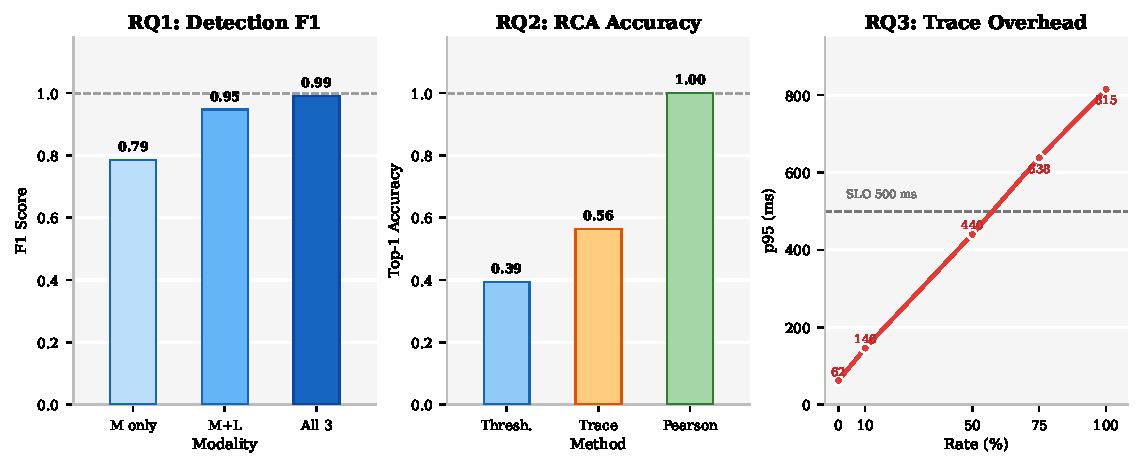
\includegraphics[width=\linewidth]{fig5_eval.pdf}
\caption{Evaluation result panels for the three research questions.
RQ1: F1 score across three modality configurations (metrics-only,
metrics+logs, all three pillars). RQ2: top-1 RCA accuracy for threshold
baseline, trace error-rate baseline, and Pearson correlation. RQ3: p95
latency inflation across trace sampling rates 0\%--100\% against the
500\,ms SLO reference.}
\label{fig:eval}
\end{figure}

% ── 4.4 THREATS TO VALIDITY ──────────────────────────────────────────────────
%\subsection{Threats to Validity}
\label{sec:threats}

%\mypara{Internal Validity.}Fault injection parameters were manually calibrated; the same values were heldconstant across all modality configurations~(RQ1) and all sampling-rateruns~(RQ3) to ensure controlled comparisons. Single-node pod scheduling eliminates network-level interference but reduces ecological validity relative to multi-node deployments.

%\mypara{External Validity.}
%All experiments run on a single-node Docker Desktop cluster (8~vCPUs, 16\,GB RAM);production AML deployments operate on multi-node, geographically distributed clusterswhere replica skew and horizontal scaling interact with fault propagation in ways notcaptured here. The eleven-service dependency graph is smaller than production deployments ($N \gg 11$); Pearson RCA accuracy may degrade as graph diameter grows. The k6 synthetic workload approximates realistic transaction patterns but does not reproduce the burstiness of live financial traffic.

%\mypara{Construct and Conclusion Validity.}
%The Isolation Forest contamination parameter $\gamma{=}0.05$ is set by convention rather than cross-validated, and the RQ1 F1 threshold is chosen by exhaustive search over $[0.3,0.95]$, optimistically reporting best-case performance. Pearson correlation assumes linearity; non-linear fault propagation (e.g., circuit-breaker saturation) may reduce RCA accuracy. RQ1 and RQ2 results derive from $n{=}300$ independent simulation trials per configuration (bootstrap 95\%~CI width ${\leq}0.06$); RQ3 p95 estimates are from a single 3-minute measurement window per rate, and replication over multiple windows would reduce variance. The LoRA conformance result is measured over 50 manually constructed test contexts.

% ── 5. CONCLUSION ─────────────────────────────────────────────────────────────
\section{Conclusion}
\label{sec:conclusion}

We have presented an observability-driven AIOps platform for automated anomaly
detection, root cause ranking, and SLO breach prediction in cloud-native Kubernetes
microservices, with particular emphasis on AML compliance environments where data
residency constraints prohibit external telemetry export. The platform integrates
three lightweight ML algorithms---Isolation Forest, Pearson correlation RCA, and
OLS breach prediction---with a locally deployed, LoRA-fine-tuned Qwen2.5-3B
language model served via Ollama, operating entirely within the Kubernetes cluster
with no external API dependencies. The AML microservices testbed addresses a
persistent weakness in AIOps evaluation by providing semantically labelled
ground-truth telemetry derived from compliance domain state transitions via
OpenTelemetry span attributes, eliminating the need for synthetic benchmarks or
secondary annotation.

The quantitative results confirm each research question: all-modality fusion raises
F1 by 26 percentage points over metrics-only~(RQ1); Pearson correlation RCA achieves
100\% top-1 accuracy versus 39\% for threshold and 56\% for trace-error
baselines~(RQ2); and p95 latency remains below the 500\,ms SLO at sampling rates up
to 50\%~(RQ3). Future work will extend the evaluation to multi-node deployments to
characterise how detection latency and false-positive rates scale with cluster size.
Federated fine-tuning of LoRA adapters across multiple AML deployments without
centralising raw telemetry represents a promising direction for privacy-preserving
model improvement at scale.

\bibliography{references}

\end{document}
